\documentclass{article}
\usepackage[margin=1.5in]{geometry}
\usepackage{graphicx} % Required for inserting images
\usepackage{amsmath}
\usepackage{amssymb}
\usepackage{amsfonts}
\usepackage{enumitem} % For pretty enumeration
\usepackage{amsthm}
\usepackage{systeme}
\usepackage{cancel}
\newtheorem{theorem}{Theorem}

% general operators
\DeclareMathOperator{\C}{\mathbb{C}}
\DeclareMathOperator{\R}{\mathbb{R}}
\DeclareMathOperator{\Z}{\mathbb{Z}}
\DeclareMathOperator{\N}{\mathbb{N}}
\DeclareMathOperator{\Q}{\mathbb{Q}}

% hw specific operators
\DeclareMathOperator{\uu}{\mathbf u}
\DeclareMathOperator{\vv}{\mathbf v}
\DeclareMathOperator{\g}{\mathbf g}
\DeclareMathOperator{\x}{\mathbf x}
\DeclareMathOperator{\y}{\mathbf y}
\DeclareMathOperator{\z}{\mathbf z}
\def\epsilon{\varepsilon}
\newcommand{\mb}{\mathbf}
\newcommand{\dotp}{\boldsymbol{\cdot}}

\title{\vspace{-0.5in}Shift Schedule Optimization}
\author{Tobias Michlik}
\date{May 13, 2026}

\begin{document}
\maketitle

\section*{Intro}
We want to find the best schedule given everyone's shift availability and preference. The result has to be valid and optimized. A valid schedule follows the following rules:
\begin{enumerate}
    \item Anyone working a shift must work its full number of hours
    \item All required shifts are filled with the right number of workers,
    \item No worker is working a shift they aren't available for, and
    \item Each shift is wholly worked by one worker. Some shifts are worth more than 1 working hour and cannot be split between workers.
\end{enumerate}
Each worker gives a preference score in $[1,10]$ for the shifts they are available for (and 0 for unavailable shifts). An optimized shift maximizes the sum of preference scores.


\section*{Variables}
Consider the following variables:
\begin{itemize}
    \item $n=\text{number of workers}$
    \item $k=\text{number of shifts}$
    \item $P\in\Z^{n\times k}$ represents worker availability and preference data:
    \begin{enumerate}[label=]
        \item $\forall\ 1\le i\le n$ and $\forall\ 1\le j\le k,$ let $0\le P_{ij}\le 10$ represent worker $i$'s preference score for shift $j$. 0 indicates a shift they aren't available for.
    \end{enumerate}
    Example:
        \[P^1=\begin{bmatrix}
            0&0&1&10\\
            2&0&3&8\\
            4&4&9&0\\
            0&0&6&0\\
            9&8&4&9
        \end{bmatrix}\]
    \item $S\in\Z^{k\times2}$ represents shift data:
    \begin{align*}
        \forall\ 1\le m\le k,\ &S_{m1}=\text{shift working hours for shift $m$}&\\
        &S_{m12}=\text{number of workers for shift $m$}&
    \end{align*}
    Example:
        \[S^1=\begin{bmatrix}
            2&1\\
            1&1\\
            1&1\\
            2&1
        \end{bmatrix}\]
    \item $x=\text{max number of hours per worker}=$
        \[\max\left(\bigg\lceil\dfrac{1}{n}\sum_{m=1}^{k}S_{m1}\cdot S_{m2}\bigg\rceil,\ \max_{1\le m\le k}S_{m1}\right)\]
    In our example, let $n_1=5$:
        \[x_1=\bigg\lceil\dfrac{1}{n_1}\sum_{m=1}^{k_1}S^1_{m1}\cdot S^1_{m2}\bigg\rceil=\max_{1\le m\le k_1}S^1_{m1}=2\]
    % \item $W\in\{0,1\}^{n\times k}$ is an indicator matrix, representing a map of shifts each worker is available for.
    % \begin{align*}
    %     \forall\ i,j,\quad W_{ij}=
    %     \begin{cases}
    %         1, & P_{ij}>0\\
    %         0, & P_{ij}=0
    %     \end{cases}
    % \end{align*}
    % Example:
    %     \[W^1=\begin{bmatrix}
    %         0&0&1&1\\
    %         1&0&1&1\\
    %         1&1&1&0\\
    %         0&0&1&0\\
    %         1&1&1&1
    %     \end{bmatrix}\]
\end{itemize}


\section*{Objective Function}
\begin{itemize}
    \item $\theta\in\R^{n\times x}$ is the input to our objective function. Let $\Theta\in\Z^{n\times x}$ be $\text{round}(\theta)$ (each element of $\theta$ is rounded to the nearest integer).
    \begin{enumerate}[label=]
        \item $\forall\ 1\le i\le n$ and $1\le j\le x$, $0\le\theta_{ij}\le k$. We get our solution by rounding each $\theta_{ij}$ to the nearest integer to get worker $i$'s $j$th assigned shift with index of $\text{round}(\theta_{ij})$. A zero represents no scheduled shift.
    \end{enumerate}
    Example:
        \[\theta^1=\begin{bmatrix}
            4.0&3.9\\
            0.0&0.3\\
            1.9&0.1\\
            3.2&0.0\\
            1.3&1.2
        \end{bmatrix}\implies\text{round}(\theta^1)=\Theta^1=\begin{bmatrix}
            4&4\\
            0&0\\
            2&0\\
            3&0\\
            1&1
        \end{bmatrix},\ \text{a valid solution.}\]
    \item $\forall\ 1\le i\le n,\ \hat P_i:[0,k]\rightarrow\R$ is a helper function to the objective function.
        \[\hat P_i(s) = (1-\alpha)P_{i\lfloor s\rfloor} + \alpha P_{i\lceil s\rceil},\quad \alpha=s-\lfloor s\rfloor\]
    \item $f(\theta):\R^{n\times x}\rightarrow\R$ is our objective function. We aim to minimize the objective function.
        \[f(\theta) = -\sum_{i=1}^{n}\sum_{j=1}^{x}\hat P_i(\theta_{ij})\]
\end{itemize}


\section*{Constraints}
\begin{enumerate}    
    \item Every shift $m$ must appear exactly $S_{m1}$ times across the entire $\Theta$ matrix. With $\mb1$ as an indicator function:
        \[\forall\ 1\le m\le k,\quad S_{m1}=\sum_{i=1}^n\sum_{j=1}^x\mb1(\Theta_{ij}=m)\hfil\tag{C1}\]
    \item Every shift $m$ must be found in $S_{m2}$ unique rows within $\Theta$:
        \[\forall\ 1\le m\le k,\quad S_{m2}=\sum_{i=1}^n\mb1\left(\sum_{j=1}^x\mb1(\Theta_{ij}=m)\ge1\right)\hfil\tag{C2}\]
    \item No worker can be assigned a shift where their preference is 0/they are unavailable:
        \[\forall\ i,j,\quad \hat P_i(\theta_{ij})>0\hfil\tag{C3}\]
    \item If any part of a shift $m$ is assigned to a worker $i$, then the entire length $S_{m1}$ must be assigned to that same worker $i$:
        \[\forall\ 1\le m\le k,\quad \exists\ 1\le i\le n\ \text{s.t.}\ S_{m1}=\sum_{j=1}^x\mb1(\Theta_{ij}=m)\hfil\tag{C4}\]
\end{enumerate}


\section*{Initial NLP}
\begin{equation*}
(Q)\qquad\left\{\begin{aligned}
    & \underset{ \mb \theta \in \R^{n\times x}}{\text{minimize}}
    & & f(\theta) \\
    & \text{subject to} && S_{m1}=\sum_{i=1}^n\sum_{j=1}^x\mb1(\Theta_{ij}=m)\quad &\forall\ 1\le m\le k\\
    &&& S_{m2}=\sum_{i=1}^n\mb1\left(\sum_{j=1}^x\mb1(\Theta_{ij}=m)\ge1\right)\quad &\forall\ m\\
    &&& \hat P_i(\theta_{ij})>0\quad &\forall\ i,j\\
    &&& \exists\ 1\le i\le n\ \text{s.t.}\ S_{m1}=\sum_{j=1}^x\mb1(\Theta_{ij}=m)\quad&\forall\ m
    \end{aligned}\right.
\end{equation*}
Ideally, we optimize a NLP without any constraints. Let's consider ways to optimize this.


\section*{Optimizing Constraints}
% \subsection*{Consolidating Constraints}
% Notice that our third constraint is very similar to the first. In it's current form, C4 isn't sufficient for C1. However, by simply adding a unique qualifier to the existence of $i$, it does become sufficient. Thus, for our first optimization, we only have C3 and the modified C4:
%     \[\forall\ 1\le m\le k,\quad \exists!\ 1\le i\le n\ \text{s.t.}\ S_{m1}=\sum_{j=1}^x\mb1(\Theta_{ij}=m).\]

% \subsection*{Penalties}
Now, we should convert our constraints into penalties.
\paragraph{Penalty$_{\mb{C1}}$}
Indicator functions aren't very good for generating continuous penalties. Our first step is to stop checking when $\Theta_{ij}=m$ and instead determine how far $\theta_{ij}-m$ is from 0. So, for each shift, instead of checking our solution has the right count of working hours for the shift, we check the sum of a continuous analogue to our indicator function. The function we'll use is kernel density estimator $K:\R^{3}\rightarrow\R$
    \[K_\sigma(\phi)=\exp\left(-\dfrac{(\phi)^2}{2\sigma^2}\right).\]
Think of it as a bell curve around with mean $0$ and variance $\sigma^2$. When optimizing:
\begin{itemize}
    \item Start with a wide $\sigma$.
    \item Gradually ramp it down.
    \item Eventually it'll force the optimizer to output near integers within $\theta$.
\end{itemize}
Now, for every shift, $m$, we sum up these densities across every assigned shift in $\theta$:
    \[C_m(\theta)=\sum_{i=1}^n\sum_{j=1}^x K_\sigma(\theta_{ij}-m).\]
With $m=3$ and $\sigma=0.5$, $C_3^1$ across all possible $\theta_{\cdot\cdot}$ values is a pointed sheet with two perpendicular ridges, as show in Figure \ref{fig:c1penalty}\\
\begin{figure}
    \centering
    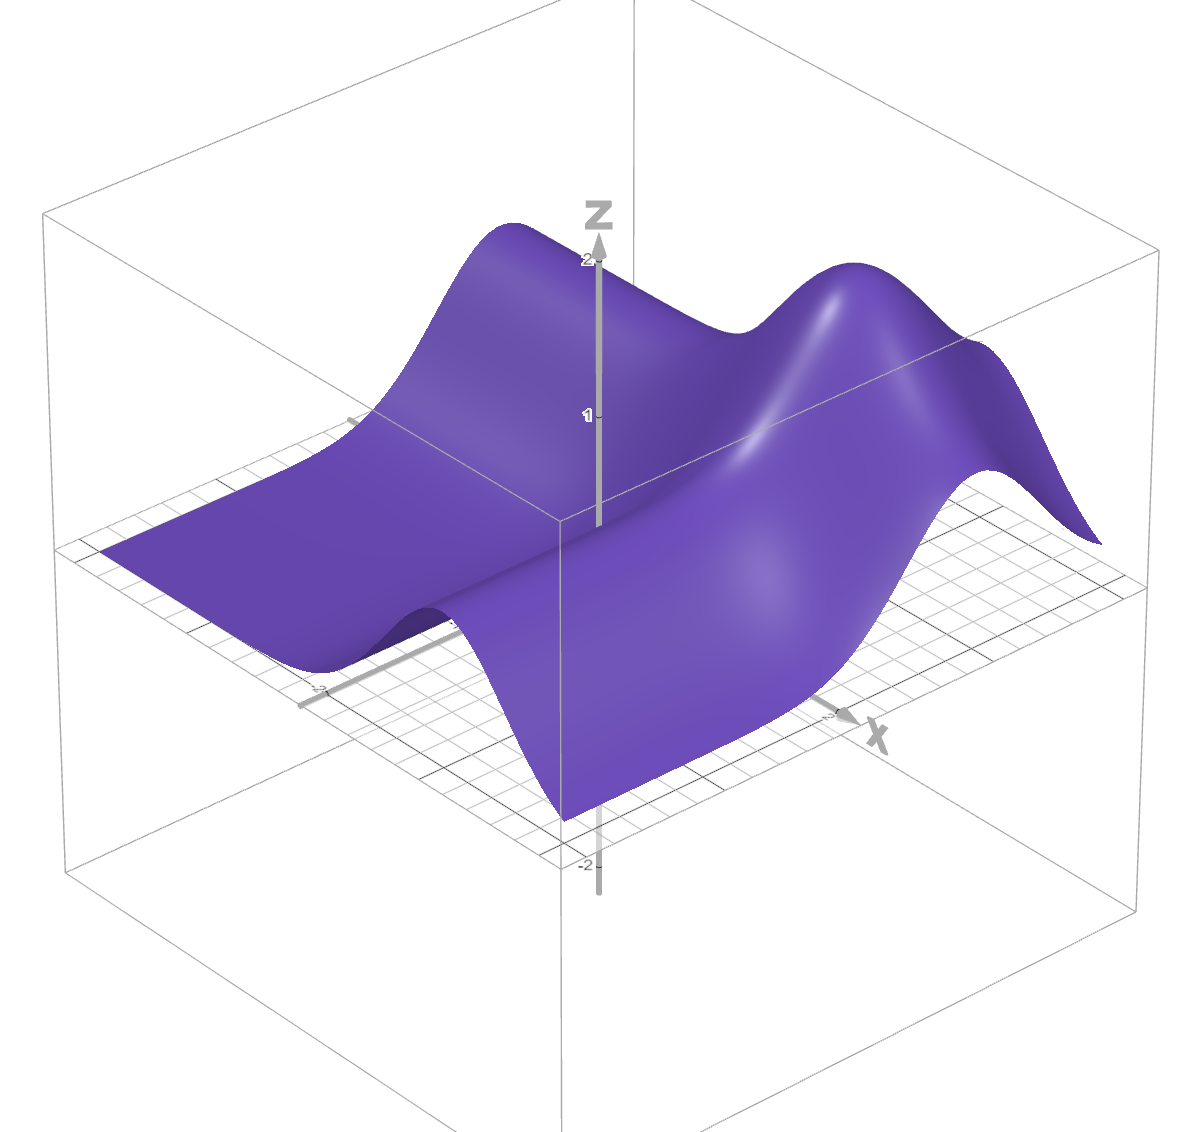
\includegraphics[width=0.5\linewidth]{C1_penalty.png}
    \caption{$C_3^1$ across all valid inputs shifted toward origin by 2 points}
    \label{fig:c1penalty}
\end{figure}
\\
Since we now have a distribution of shift coverage, for each shift, we have to test if it's been covered properly. To do so, we compare the difference between the coverage score and shift working hours:
    \[\text{Penalty}_{C1}=\sum_{m=1}^k\big(C_m(\theta)-(S_{m1}\cdot S_{m2})\big)^2.\]
If a shift is over- or under-assigned, there is a positive penalty.

\paragraph{Penalty$_{\mb{C2}}$}
Since a worker can only work 1 role in a shift, they cannot exceed working the base shift duration. Thus, we penalize whenever a worker's work duration for a shift exceeds the shift duration. Consider the shift coverage score \textit{per worker}:
    \[C_{i,m}(\theta)=\sum_{j=1}^xK_\sigma(\theta_{ij}-m).\]
We apply a hinge loss penalty:
    \[\text{Penalty}_{C2}=\sum_{m=1}^k\sum_{i=1}^n\max(0,C_{i,m}(\theta)-S_{m1})^2\]

\paragraph{Penalty$_{\mb{C3}}$}
With C3 as $\hat P_{i}(\theta_{ij})>0$, we need a big penalty as $\hat P_i$ gets near 0. To do so, we apply a hinge loss, penalizing when preference score falls below $\tau$:
    \[\text{Penalty}_{C3}=\sum_{i=1}^n\sum_{j=1}^x\max(0,\tau-\hat P_i(\theta_{ij}))^2,\quad\tau=1\]
In this case, $\tau$ can be set to 1 since we don't want to be assigning unavailable shifts which have preference score below 1.

\paragraph{Penalty$_{\mb{C4}}$}
We can do a very similar thing for $C4$ as for $C1$. The difference is that we're primarily checking each worker covers the full hours of their assigned shift. We need to penalize whenever a worker has neither the full shift ($S_{m1}$) nor none of it (0).\\\\
Using the same square error, we can penalize deviance from a worker having less parts of a shift. The square of the coverage score penalizes having the shift. These together makes the desired effect.
    \[\text{Penalty}_{C4}=\sum_{m=1}^k\sum_{i=1}^n\big[C_{i,m}(\theta)^2\cdot(C_{i,m}(\theta)-S_{m1})^2\big].\]

\paragraph{Total Penalty}
When we put out penalties together, we use 4 hyperparameters to control the strength of the corresponding penalty terms:
    \[\lambda_1\text{Penalty}_{C1}+\lambda_2\text{Penalty}_{C2}+\lambda_3\text{Penalty}_{C3}+\lambda_4\text{Penalty}_{C4}.\]
Tuning these is a bit of a task, but here are included some techniques varying in sophistication. And don't forget to tune $\sigma$ (potentially distinct within Penalty$_{C1}$ and Penalty$_{C4}$).
\begin{enumerate}
    \item Grid Search:
    \begin{itemize}
        \item We select $\lambda_i=10^\alpha$, $\alpha\in[-4,4]$.
        \item Run the optimization for each combination
        \item Evaluate preference score, scheduling violations, and atomic coverage error.
        \item Select best $\lambda$s.
    \end{itemize}
    \item Better yet is to treat $\lambda$s as hyperpriors in a Bayesian model. We put priors on $\lambda$s and infer them by sampling.
    \item Adaptive Tuning: Start with small penalties and
    \begin{itemize}
        \item increase them as optimization progresses,
            \[\lambda_i^{(t+1)}=\gamma\lambda_i^{(t)},\quad\gamma>1,\]
        or
        \item update them based on constraint violations,
            \[\lambda_i^{(t+1)}=\lambda_i^{(t)}+\rho\cdot\text{violation},\quad\rho>1.\]
    \end{itemize}
\end{enumerate}


\section*{Final NLP}
Since we have converted our constraints all into penalties, we can write our final objective function as a single continuous and piecewise differentiable function.
    \[(Q)\qquad\begin{cases}\underset{ \mb \theta \in \R^{n\times x}}{\text{minimize}}\quad f(\theta)+\lambda_1\text{Penalty}_{C1}+\lambda_2\text{Penalty}_{C2}+\lambda_3\text{Penalty}_{C3}+\lambda_4\text{Penalty}_{C4}\end{cases}\]


\end{document}